\chapter{Establishing secure communication channel}

\section{Encryption}

Encryption is the original goal of cryptography. It is the process of encoding messages in such a way that only authorized parties can read it. Encryption does not of itself prevent interception, but denies the message content to the interceptor.

The generic use case is: Alice and Bob\footnote{Alice, Bob and Eve are placeholder names commonly used when discussing cryptography, to identify an archetypal role of participant. Alice is a sender, Bob is a receiver and Eve is an eavesdropper. For the first time these names were used in Ron Rivest's paper introducing RSA public key cryptosystem \todo{Ref it}. Since then, a number of other names have entered cryptographic literature.} want to communicate with each other. However, communication channels are assumed not to be secure. Eve is eavesdropping on the channel. Any message that Alice sends to Bob is also received by Eve. (The same applies for messages sent from Bob to Alice, but it is the same problem and the same solution will work for Bob's messages, so we concentrate to Alice messages.) How can Alice and Bob communicate without learning everything? (\autoref{img:encryption_problem}) \cite[p.~23]{ferguson2010cryptography}

To prevent Eve from understanding the conversation, Alice and Bob are using encryption (\autoref{img:encryption}). They first agree on a cipher and a secret key. The secret key needs to be exchanged via some secure communication channel that Eve cannon eavesdrop on. Alice and Bob can meet in person to exchange the key, or Alice can mail it via public post service.

\begin{figure}
  \centering
  \begin{tikzpicture}
    \node (alice) at (0,0) [rect,label=below:{Alice}] {$m$};
    \node (bob) at (8,0) [rect,label=below:{Bob}] {$m$};
    \node (eve) at (4,-1) [rect,label=below:{Eve},label=right:{\noMark}] {$m$};
    \coordinate (channel) at (4,0);
    \draw [->,thick] (alice) -- (bob) node[pos=0.15,above]{$m$};
    \draw [->,thick,rounded corners] (alice) -- (channel) -- (eve);
  \end{tikzpicture}
  \caption{How can Alice and Bob communicate securely?}
  \label{img:encryption_problem}
\end{figure}

\begin{figure}
  \centering
  \begin{tikzpicture}
    \node (alice) at (0,0) [rect,label=below:{Alice}] {$m, c := E(K_e, m)$};
    \node (bob) at (8,0) [rect,label=below:{Bob}] {$c, m := D(K_e, c)$};
    \draw [->,thick] (alice) -- (bob) node[pos=0.15,above]{$c$};
  \end{tikzpicture}
  \caption{Generic setting for encryption}
  \label{img:encryption}
\end{figure}

\begin{figure}
  \centering
  \begin{tikzpicture}
    \node (alice) at (0,0) [rect,label=below:{Alice}] {$m$};
    \node (bob) at (8,0) [rect,label=below:{Bob},label=right:{\noMark}] {$m'$};
    \node (eve) at (4,-1) [rect,label=below:{Eve}] {$m'$};
    \coordinate (channel) at (4,0);
    \draw [->,thick] (alice) -- (channel) node[pos=0.3,above]{$m$};
    \draw [->,thick,rounded corners] (eve) -- (channel) -- (bob) node[pos=0.85,above]{$m'$};
  \end{tikzpicture}
  \caption{How does Bob know who sent the message?}
  \label{img:authentication_problem}
\end{figure}

\begin{figure}
  \centering
  \begin{tikzpicture}
    \node (alice) at (0,0) [rect,label=below:{Alice}] {$m, a := H(K_a, m)$};
    \node (bob) at (8,0) [rect,label=below:{Bob}] {$m, a \stackrel{?}{=} H(K_a, m)$};
    \draw [->,thick] (alice) -- (bob) node[pos=0.15,above]{$m, a$};
  \end{tikzpicture}
  \caption{Generic setting for authentication}
  \label{img:authentication}
\end{figure}

\begin{figure}
  \centering
  \begin{tikzpicture}
    \node (alice) at (0,0) [rect,label=below:{Alice}] {$m, c := E(PK_{Bob}, m)$};
    \node (bob) at (8,0) [rect,label=below:{Bob}] {$c, m := D(SK_{Bob}, c)$};
    \draw [->,thick] (alice) -- (bob) node[pos=0.15,above]{$c$};
  \end{tikzpicture}
  \caption{Generic setting for public-key encryption}
  \label{img:authentication}
\end{figure}

\begin{figure}
  \centering
  \begin{tikzpicture}
    \node (alice) at (0,0) [rect,label=below:{Alice}] {$m, a := S(SK_{Alice}, m)$};
    \node (bob) at (8,0) [rect,label=below:{Bob}] {$m, V(PK_{Alice}, m, a) ?$};
    \draw [->,thick] (alice) -- (bob) node[pos=0.15,above]{$m, a$};
  \end{tikzpicture}
  \caption{Generic setting for digital signature}
  \label{img:authentication}
\end{figure}


\chapter{Authenticated Encryption}

\todo{popis AEAD}

\section{Block cipher modes}

from 70s

\begin{description}
  \item[ECB]
  \item[CBC]
  \item[CFB]
  \item[OFB]
  \item[CTR]
\end{description}

\todo{Block cipher modes image from @angealbertini}

Exploiting malleability:

ECB: Rearrange, replay blocks
CTR, OFB: Bitwise modification of blocks
CBC: Change current ciphertext block to predictably change the next plaintext block (during decryption)

Chosen-boundary attacks:

ECB, CBC, CFB: Partial chosen-plaintext control
Decrypt messages byte by byte

Here come the XOR ninjas

\section{Authenticated Encryption}
\section{Authenticated Encryption with Associated Data}



\section{Generic compositions}

\begin{description}
  \item[Encrypt-and-MAC]
  \item[MAC-then-Encrypt]
  \item[Encrypt-then-MAC]
\end{description}

\begin{figure}
  \centering
  \begin{subfigure}[b]{0.3\textwidth}
    \centering
    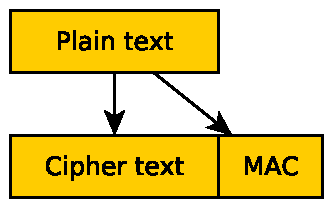
\includegraphics[width=0.9\textwidth]{images/encrypt-and-mac.pdf}
    \caption{Encrypt-and-MAC}
  \end{subfigure}
  \begin{subfigure}[b]{0.3\textwidth}
    \centering
    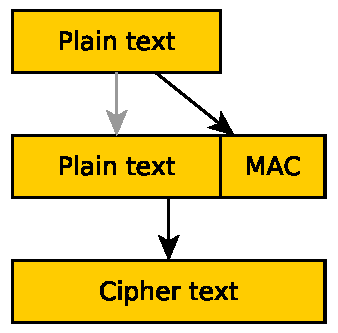
\includegraphics[width=0.9\textwidth]{images/mac-then-encrypt.pdf}
    \caption{MAC-then-encrypt}
  \end{subfigure}
  \begin{subfigure}[b]{0.3\textwidth}
    \centering
    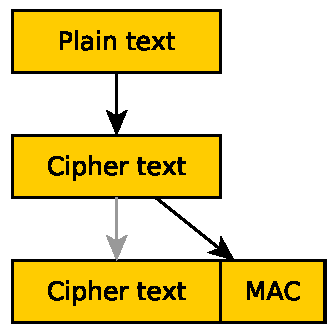
\includegraphics[width=0.9\textwidth]{images/encrypt-then-mac.pdf}
    \caption{Encrypt-then-MAC}
  \end{subfigure}
  \caption{Generic compositions of Authentized Encryption}
\end{figure}

\section{Competition for Authenticated Encryption: Security, Applicability and Robustness}

CAESAR is worldwide cryptographic competition, focused on finding new methods of authenticated encryption, that offer advantages against commonly used AES-GCM and will be suitable for widespread adoption. Submitted algorithms will be publicly evaluated by committee of researchers in fields of cryptography and cryptoanalysis.

\todo{popis algoritmů byly v soutěži, v čem se lišily, jaké a jak v nich byly nalezeny zranitelnosti a proto nepostoupily}

\todo{výběr algoritmu pro implementaci}

\subsection{Selection criteria}

\begin{description}
  \item[Online (one-pass)]
\end{description}



\subsection{NORX}

NO(T A)RX

ARX - Addition, Rotation, XOR

\subsubsection{Design goals}

\begin{itemize}
  \item \textbf{High security}
  \item \textbf{High speed} (in SW \textit{and} HW)
  \item \textbf{Simplicity} (of spec \textit{and} code)
  \item Online / one-pass
  \item Scalability (parallelism, unrolling)
  \item High key agility (no "key schedule")
  \item Side-channel leaks robustness (esp. timings)
\end{itemize}

\subsubsection{Parameters}

\begin{description}
  \item[Word Bit Size] $W \in {32, 64}$
  \item[Number of Rounds] $1 \leq R \leq 63$
  \item[Parallelism Degree] $0 \leq D \leq 255$ (0?)
  \item[Tag Bit Size] $|A| \leq 10W$
\end{description}

\begin{table}
  \centering
  \csvreader[
    after head=\begin{tabular}{llll}\toprule\csvlinetotablerow\\\midrule,
    late after line=\\,
    late after last line=\\\bottomrule\end{tabular}
  ]
    {tables/norx-proposed-instances.csv}{}
    {\texttt{\csvcoli} & \csvcolii & \csvcoliii & \csvcoliv}

  \caption{NORX proposed instances}
\end{table}

R=6: higher security margin

D=4: high throughput on parallel architectures

\subsection{Selection}

Benchmarks - Supercop, Brutus

\url{https://eprint.iacr.org/2014/850.pdf}
\url{http://www1.spms.ntu.edu.sg/~syllab/speed/}



